% Capítulo 2
\chapter{Capítulo 2}

Neste capítulo, descreve-se o funcionamento do módulo \textit{glycowork.motif.regex}, suas funções principais, a atuação das expressões regulares e as vantagens do uso desse sistema.

O módulo \textit{glycowork.motif.regex}, introduzido por Bennett e Bojar (2024) no pacote \textit{glycowork}, representa um avanço significativo na análise computacional de glicanos ao incorporar o uso de expressões regulares (RegEx) para identificação e extração de padrões estruturais complexos. Essa abordagem adapta a lógica das RegEx convencionais, amplamente utilizadas em ciência da computação, para detecção de padrões em cadeias de texto, ao contexto estrutural e não linear dos glicanos, permitindo buscas mais precisas e flexíveis em sequências de carboidratos.

\section{Estrutura e funções do módulo}

O módulo foi desenvolvido para permitir que pesquisadores expressem padrões estruturais de glicanos em uma forma análoga às expressões regulares de texto. Ele se baseia na tradução de padrões definidos em formato de expressão regular para operações de isomorfismo de subgrafos dentro das estruturas moleculares de glicanos. Quando o usuário fornece um padrão, por exemplo, um motivo glicosídico como \texttt{Neu5Ac$\alpha$2-3Gal$\beta$1-4(Fuc$\alpha$1-3)GlcNAc}, o sistema decompõe esse padrão em unidades menores, chamadas de módulos homogêneos, correspondentes a monossacarídeos e ligações individuais. Cada módulo é então processado para identificar as possíveis correspondências no grafo do glicano, permitindo localizar subestruturas equivalentes de forma independente da forma textual em que o glicano foi representado. Isso é essencial, já que o módulo aceita múltiplos formatos de entrada, como WURCS, GlycoCT, Oxford, IUPAC-condensed e outras notações padronizadas.

As expressões regulares glicosídicas seguem uma lógica análoga à das regex textuais, com suporte a modificadores, quantificadores e operadores de busca contextual, como \textit{lookahead} e \textit{lookbehind}. Isso permite definir quantas vezes um determinado monossacarídeo pode aparecer, se uma ligação é opcional ou se uma ramificação deve ocorrer em uma posição específica. O sistema aceita curingas, como o caractere “.” ou o termo \texttt{Monosaccharide}, que funcionam como substitutos para qualquer unidade estrutural. Os ramos das moléculas são representados por parênteses, e ligações específicas podem ser explicitadas, como em \texttt{Mana6} ou \texttt{Galb3/4}, o que permite uma descrição sintática detalhada da estrutura. Após o processamento dos módulos e operadores, o sistema percorre o grafo da molécula para traçar um caminho contínuo que satisfaça todas as condições da expressão regular, retornando as correspondências encontradas. Por padrão, o comportamento é “guloso”, ou seja, o sistema tenta encontrar o maior padrão possível, embora a execução “preguiçosa”, que busca o menor padrão que satisfaça a condição, também seja suportada com o modificador “?”.

Entre as principais funções do módulo destacam-se:
\begin{itemize}
   \item \texttt{get\_match()}: Busca e extrai trechos da estrutura do glicano que correspondem a um padrão definido pelo usuário.
   \item \texttt{get\_pvals\_motifs()}: Avalia o enriquecimento estatístico de motivos dentro de diferentes contextos estruturais, permitindo identificar padrões recorrentes em conjuntos de glicanos.
   \item \texttt{get\_differential\_expression()}: Analisa a expressão diferencial de motivos glicosídicos entre grupos de amostras, facilitando a identificação de variações significativas em estudos comparativos.
\end{itemize}

Essas funções se integram diretamente às demais ferramentas do pacote \textit{glycowork}, como a \texttt{GlycoDraw}, que permite visualizar graficamente os motivos identificados, e os módulos de anotação e destaque de redes de motivos. Essa integração favorece a análise automatizada e a exploração visual das estruturas reconhecidas pelas expressões regulares.

A seguir, apresenta-se um exemplo ilustrativo de inclusão de figura no contexto do módulo.

\begin{figure}[htb]
	\centering
  	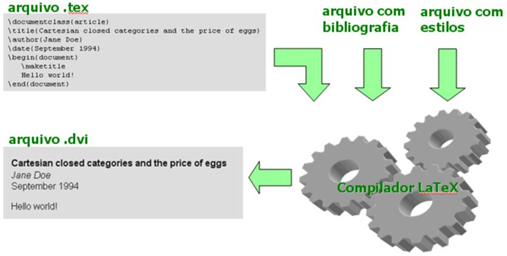
\includegraphics[scale=0.75]{Imagens/FiguraTeste.png}
  	\textsf{\caption{Teste de uma figura em formato .png.}}
  	\label{fig:FiguraTeste}
\end{figure}

\section{Operação interna e papel das expressões regulares}

O funcionamento interno do módulo envolve a tradução de padrões \textit{RegEx} em operações de subgrafo sobre as estruturas moleculares representadas como grafos. Em termos gerais, o processo é dividido em etapas sucessivas que permitem converter descrições simbólicas de ligações e unidades monossacarídicas em estruturas compreensíveis computacionalmente.

Primeiramente, ocorre a segmentação do padrão, na qual a expressão \textit{RegEx} fornecida é decomposta em módulos homogêneos, como unidades monossacarídicas ou ligações específicas. Por exemplo, o padrão \texttt{"Neu5Ac$\alpha$2-3Gal$\beta$1-4(Fuc$\alpha$1-3)GlcNAc"} é dividido em blocos como \texttt{"Neu5Ac$\alpha$2-3"}, \texttt{"Gal$\beta$1-4"} e \texttt{"Fuc$\alpha$1-3"}, representando diferentes segmentos estruturais que serão posteriormente analisados. Em seguida, ocorre a interpretação e expansão dos modificadores e quantificadores. Operadores como \texttt{+}, \texttt{*}, \texttt{?}, intervalos \texttt{\{m,n\}} e quantificadores preguiçosos (\texttt{+?}) são suportados, permitindo definir repetições, ocorrências opcionais ou faixas de aparecimento dos motivos. Essa flexibilidade amplia a capacidade do módulo de reconhecer variações estruturais dentro de uma mesma família de glicanos. Posteriormente, aplica-se o processo de \textit{subgraph isomorphism}, em que cada segmento é buscado dentro do grafo que representa a estrutura glicosídica. Essa etapa utiliza algoritmos de isomorfismo de subgrafos para identificar correspondências exatas, mesmo em representações complexas que envolvem ramificações e múltiplas conexões entre unidades.

Outro componente essencial é a implementação das operações de \textit{lookahead} e \textit{lookbehind}, herdadas das expressões regulares textuais. Elas permitem incluir ou excluir determinados contextos do padrão de busca sem incorporá-los ao resultado final, sendo cruciais para capturar motivos cuja ocorrência depende de um contexto estrutural específico.

Por fim, ocorre a construção do caminho de correspondência, na qual um algoritmo iterativo reconstrói o trajeto contínuo dentro do grafo, unindo as correspondências parciais e validando os requisitos definidos pela expressão completa. Essa abordagem possibilita representar ligações específicas, como $\alpha$1-3 ou $\beta$1-6, bem como ambiguidade estrutural e ramificações expressas por meio de parênteses. Dessa forma, a notação \textit{RegEx} é adaptada à topologia molecular, permitindo uma modelagem altamente expressiva e precisa das estruturas glicosídicas.

\section{Benefícios e ganhos do uso de regex em glicobiologia computacional}


\section{Considerações finais}

